\begin{figure*}[t]
	\centering
	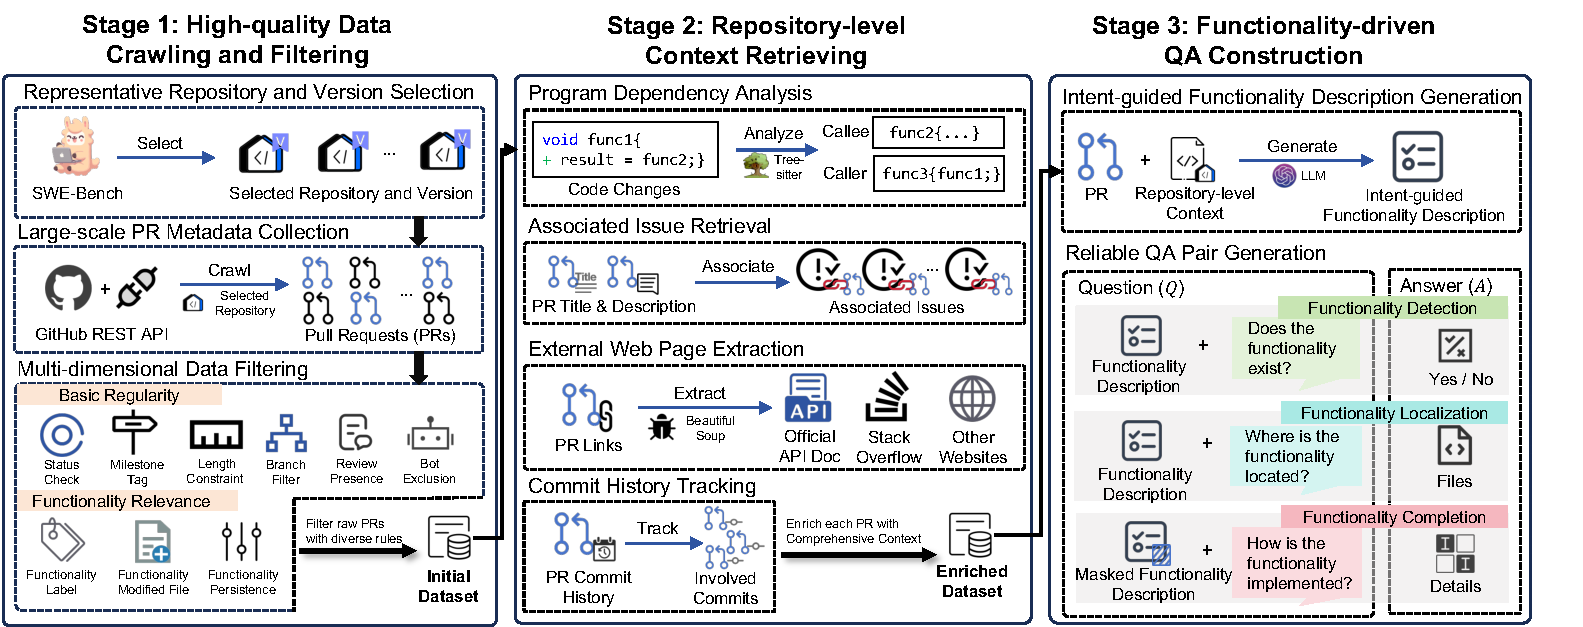
\includegraphics[width=\textwidth]{Figures/framework.pdf}
    \vspace{-2em}
    \caption{The overview of \benchmark's data construction pipeline.}
\label{fig:framework}
\vspace{-1em}
\end{figure*}

We formulate the evaluation on \benchmark as a documentation-based QA problem. Let $\mathcal{D}$ denote the space of generated software documentation and $\mathcal{Q}$ be the set of potential developers' questions. The target model is defined as a function $M: \mathcal{D} \times \mathcal{Q} \rightarrow \mathcal{A}$, which takes the documentation $D \in \mathcal{D}$ and a specific question $Q \in \mathcal{Q}$ as input, and produces an answer $A \in \mathcal{A}$. The structure of the question $Q$ and the domain of the answer space $\mathcal{A}$ vary across the three tasks, as detailed below.

\subsection{Functionality Detection}
    Software documentation supports developers in identifying which functionalities are implemented within the repository. This task reflects documentation’s completeness in presenting repository functionalities. In this task, the question $Q_{\text{detect}}$ inquires about the existence of a specific functionality. The answer space $\mathcal{A}$ is binary, \ie, $\mathcal{A} = \{\text{True}, \text{False}\}$. The model output $y = M(D, Q_{\text{detect}})$ indicates whether the functionality is judged to be available.

\subsection{Functionality Localization}
    Software documentation helps developers effectively locate the source files responsible for implementing specific functionalities. This task reflects the documentation’s helpfulness in navigation and localization. Here, the question $Q_{\text{localize}}$ asks for the implementation location of a functionality. The answer space $\mathcal{A}$ corresponds to the power set of all file paths in the repository. The model predicts a list of files $F = M(D, Q_{\text{localize}})$ responsible for the functionality.

\subsection{Functionality Completion}
    Software documentation enables developers to obtain clear technical details about specific functionalities. This task reflects the documentation’s comprehensiveness in describing the functionalities' implementation details. Specifically, the question $Q_{\text{complete}}$ is formulated as a cloze-style prompt containing masked placeholders. The answer space $\mathcal{A}$ consists of sequences of details (e.g., API parameters). The model generates the missing details $T = M(D, Q_{\text{complete}})$ to complete the masked placeholders.